\documentclass[a4paper,11pt]{article}
\usepackage[utf8]{inputenc}


%%%%%%%%%%%%%%%%%%%%%%%%%%%%%%%%%%%%%%%%%%%%%%%%%%%%%%%%%%%%%%%%%%%%%%%%%%
% Hier kommen Einstellungen

% Seitenränder
\usepackage{geometry}
\geometry{
 a4paper,
 left=30mm,
 right=30mm,
 top=35mm,
 bottom=35mm,
}

\usepackage{amssymb, amsfonts, amsbsy, amsmath, amsthm}
\usepackage[ngerman]{babel}

% Bibliographie
\usepackage[style=alphabetic]{biblatex}
\usepackage[german=quotes]{csquotes}
\addbibresource{literatur.bib}

% Graphik und kommutative Diagramme
\usepackage{graphicx}
\usepackage{tikz}
\usepackage[all,cmtip]{xy}

% Etwas Farbe, man kann sogar per rgb Wert definieren
\usepackage{color}
\newcommand{\black}{\color{black}}
\newcommand{\red}{\color{red}}
\newcommand{\green}{\color{dgreen}}
\newcommand{\blue}{\color{blue}}
\newcommand{\magenta}{\color{magenta}}
\definecolor{darkblue}{rgb}{0,0,.5}

% Das macht, dass man im pdf auf die Verweise klicken kann
\usepackage[colorlinks,linkcolor=darkblue,citecolor=darkblue,urlcolor=darkblue]{hyperref}

% Fuer Randbemerkungen
\usepackage{marginnote}
\usepackage[color]{changebar}
\changebarsep0.2cm
\changebarwidth0.03cm
\cbcolor{red}


% Ringe und Körper
\newcommand{\N}{{\mathbb N}}
\newcommand{\Z}{{\mathbb Z}}
\newcommand{\Q}{{\mathbb Q}}
\newcommand{\R}{{\mathbb R}}
\newcommand{\C}{{\mathbb C}}

% Potenzmenge
\renewcommand{\P}{{\mathfrak P}}

% Abbildungen
\newcommand{\id}{\operatorname{id}}
\newcommand{\Abb}{\operatorname{Abb}}

% Theorem Definitionen mit durchlaufender Numerierung
\swapnumbers
\theoremstyle{definition}
\newtheorem{definition}[equation]{Definition}
\theoremstyle{plain}
\newtheorem{remark}[equation]{Bemerkung}
\newtheorem{example}[equation]{Beispiel}
\newtheorem{proposition}[equation]{Proposition}
\newtheorem{lemma}[equation]{Lemma}
\newtheorem{theorem}[equation]{Satz}
\newtheorem{algorithm}[equation]{Algorithmus}
\newtheorem{corollary}[equation]{Korollar}
\newtheorem{assumption}[equation]{Annahme}
\newtheorem{axiom}[equation]{Axiom}

% Beweise
\renewcommand{\proofname}{Beweis}


%%%%%%%%%%%%%%%%%%%%%%%%%%%%%%%%%%%%%%%%%%%%%%%%%%%%%%%%%%%%%%%%%%%%%%%%%%
% Jetzt kommt der Text

\begin{document}

\title{Hier kommt der Titel hin}
\author{Name des Autors}
\date{\today}

\maketitle


\begin{abstract}
   Hier kann eine kleine Zusammenfassung der Arbeit stehen.
\end{abstract}


\section{Name dieses Abschnitts}
\label{sectionx}

In dieser Arbeit soll der folgende Satz bewiesen werden.

\begin{theorem} \label{thm::bla} 
   Hier der wichtige Satz. $f = \id_X$.
\end{theorem}


\section{Name dieses Abschnitts}
\label{sectiony}

Wir nehmen Bezug auf Satz~\ref{thm::bla} in 
Abschnitt~\ref{sectionx}.
% Das ist ein Kommentar. Das tilde verhindert, dass
% bei u.U. ein Zeilenumbruch zwischen Satz und Nummer stattfindet.

\begin{proposition} \label{prop1} 
   Hier ein paar Voraussetzungen. Zum Beispiel: Seien $V$ und $W$ zwei endlich-dimensionale Vektorräume über dem Körper $K$ mit $\dim(V) = \dim(W)$.
  \begin{enumerate}
  \item Erste Aussage. Zum Beispiel: Dann sind $V$ und $W$ isomorph.
  \item Zweite Aussage. \dots
  \end{enumerate}
\end{proposition}

\begin{proof}
  Hier der Beweis der Proposition. Beweise werden immer zwischen \verb!\begin{proof}! und 
  \verb!\end{proof}! geschrieben.
  
   Zu 1. Bla
   
   Zu 2. Bla
\end{proof}

Hier der Beweis vom Satz.

\begin{proof}[Beweis von Satz~\ref{thm::bla}]
  Argumente, Argumente ...
\end{proof}


\begin{remark}
   Eine wichtige Bemerkung, die eine Nummer bekommen soll.
\end{remark}

\begin{example}
   Eine wichtiges Beispiel.
\end{example}


\section{Name dieses Abschnitts}
\label{sectionz}

\subsection{Unterabschnitt}

Hallo.

\subsubsection{Unterunterabschnitt}
\label{subsubsectionx}

Bla. 

\subsection{Unterabschnitt}

In Abschnitt~\ref{subsubsectionx} steht nicht viel.

\bigskip

\cbstart \marginnote{\red Unklar!}
Hier mal eine Fußnote\footnote{Das ist der Fußnotentext.} Werden in
Mathe aber eher selten benutzt. Hilfreich um im Text offene Fragen
etc. zu markieren, sind aber Marginnotes.  
Der Rand ist in dieser Vorlage aber eng, daher nicht viel Platz.
\cbend

\section{Formelübungen}
\label{sectionu}

$\N$, $\Z$, $\R$, $\C$, $\R^n$. $a \in X$, $b \not\in Y$, $Z \ni
z$.
$\leq$, $<$, $\geq$, $>$, $\neq$, $\subseteq$, $\supseteq$,
$\subsetneq$, $\not\subseteq$.

\medskip

\noindent
$a_1, \dots, a_n$. $b_1 \cdot b_2$. $b_1 \cdot \dots \cdot b_m$.

\medskip

\noindent
$\cup_{i \in I} A_i$, $\cap_{i \in I} B_i$. $\varnothing$,
$\emptyset$. $A \backslash B$.

\medskip

\noindent
$\hat{a}$, $\overline{a}$, $\bar{a}$. $\hat{aaa}$, $\overline{aaa}$,
$\bar{aaa}$. $\widehat{aaa}$. $\underline{bbb}$.

\medskip

\noindent
Wenn Umlaute mal nicht klappen: \"a, \"u, \ss{}.

\medskip

\noindent
$f \in \Abb(X, Y)$. $\forall$, $\exists$.

\medskip

\noindent
$$\lim_{i \rightarrow \infty} a_i = a.$$

\medskip

\noindent
Es gilt \begin{align*} a & = b = c \\ & = d = e \\ & = z.
\end{align*}

\medskip

\noindent
Es gilt \begin{align} \notag a & = b = c \\ \label{eq3} & = d = e \\
\notag & = z.
\end{align}
In Gleichung~\eqref{eq3} steht was.

\medskip

\noindent
$X^Y$. $X_i^j$. $X^{a,b,c,d,e}_{1,2,3,4}$.

\medskip

\noindent
$$\begin{pmatrix} 1 & 2  & 3 \\ 4 & 5 & 6 \end{pmatrix}$$
$f : V \rightarrow W$. $f^{-1}$.

\medskip

\noindent
$$M := \{ i \,|\, i \text{ ist Primzahl} \}, \quad \P(M).$$


\medskip

\noindent
$\alpha$, $\beta$, $\gamma$, $\Gamma$, $\Xi$.

\medskip

\noindent

Klammern $$\left [ \Bigl( \bigl\{ \{ \} \bigr) \Bigr\} \right ] $$

\medskip

\noindent
$$\frac{a}{b}, \quad \frac{ \frac{2}{3} + \prod_{i=-1}^3 a_i}{ \frac{4}{5} }$$


\medskip

\noindent
Vordefiniert: $\det$, $\lim$, $\deg$


\medskip

\noindent
Eine exakte Sequenz
\begin{align} \label{eq::raycl} 
1 \longrightarrow R^\times \overset{\alpha}{\longrightarrow} (R
/ m R)^\times \overset{\beta}{\longrightarrow} S
\overset{\gamma}{\longrightarrow} T \longrightarrow 1,
\end{align}

\medskip

\noindent
Ein kommutatives Diagramm
\begin{align}\label{diag::ar}\begin{gathered}
\xymatrixcolsep{5pc}\xymatrixrowsep{2pc}\xymatrix{ 
  V \ar[r]^{A} \ar[d]^{\pi} \ar[dr] \ar@/^2pc/[r]^{d}  & W \ar[d]^{\text{res}} \\
  V/U \ar[r]^{B} & L. }
\end{gathered}\end{align}

\section{Graphiken}
\label{sectiong}

Man kann ein Bild per Hand malen, einscannen (z.B. als jpg), und dann
einbinden. Das sieht dann so aus wie in Abbildung~\ref{fig::eins}.

\begin{figure}[h] \label{fig::eins}
\begin{center}
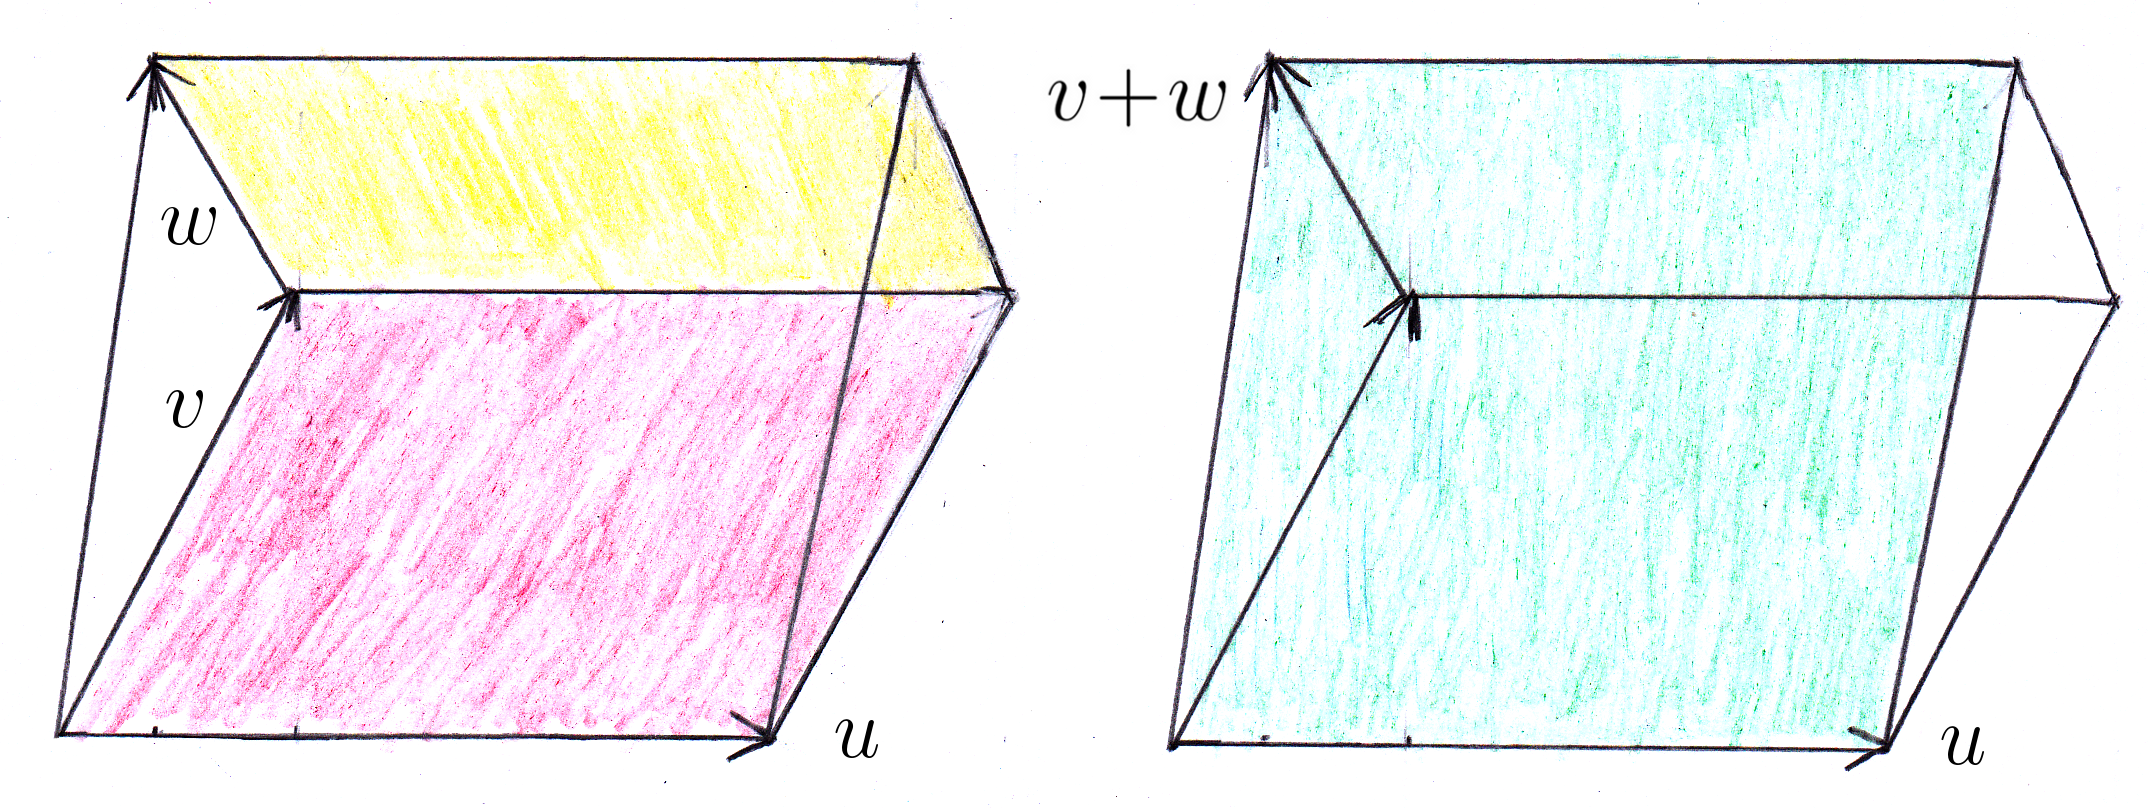
\includegraphics[scale=0.6]{voladd.png}
\end{center}
\caption{Ein illustratives Bild}
\end{figure}

Oder man malt ein Bild mit Malbefehlen, was aber oft aufwendig
ist. Ein Beispiel findet sich in Abbildung~\ref{fig::zwei} auf
Seite~\pageref{fig::zwei}.  Das wird im Overleaf Viewer aber nicht
ganz richtig angezeigt. Zum Vergleich als pdf herunterladen und so
anschauen ... Weitere Beispiele siehe
\href{http://www.texample.net/tikz/examples/all/}{TikZ} (auf TikZ
klicken!).


\begin{figure}[ht] \label{fig::zwei}
\begin{center}
\begin{tikzpicture}
  \begin{scope}[blend group = soft light]
    \fill[red!30!white]   ( 90:1.2) circle (2);
    \fill[green!30!white] (210:1.2) circle (2);
    \fill[blue!30!white]  (330:1.2) circle (2);
  \end{scope}
  \node at ( 90:2)    {Typography};
  \node at ( 210:2)   {Design};
  \node at ( 330:2)   {Coding};
  \node [font=\Large] {\LaTeX};
\end{tikzpicture}
\end{center}
\caption{Noch ein illustratives Bild mittels TikZ}
\end{figure}


\section{Benutzung der Bibliographie}

Die Daten der Quellen werden in die Datei {\tt literatur.bib}
eingetragen. Dann zitiert man so: \cite{Jech}. Oder so
\cite[S. 320]{Bosch}, \cite{Hess}, \cite{dtv}.

Tipp (für später): Wenn man MathSciNet oder das Zentralblatt zur
Literaturrecherche verwendet, kann man sich meistens die Daten für die
{\tt .bib} Dateien runterladen und muss sie nicht extra eingeben, was
sehr bequem ist.

\printbibliography


\end{document}


Was hier noch kommt wird ignoriert.


